\chapter{Euler Paths/Cycles}

Ajur was tired after listening to a lot of definitions and examples. He complained to Jura that it looked too much like a Math class and he preferred fun Math problems instead. As Ajur was mentioning, Rishnak was overhearing this conversation. Rishnak too felt that the previous day's conversation was very cut and dry. His ghost friends were accusing of making the beautiful subject of Graph Theory dull and monotonous.


An Euler walk of a connected graph is a walk that includes every edge exactly once. If the starting vertex and the ending vertex are the same then it is called a closed Euler walk. Of course the name Euler comes from Leonhard Euler.
Rishnak decided to take on the oldest problem on Graph Theory: Euler walk and closed Euler walk. Rishnak caught up with Ajur and Jura walking along a desolate road. Rishnak asked Ajur in  Figure \ref{4g1} whether there is a walk starting from vertex 2 to vertex 4 passing all the edges exactly once [This is what is known as an Eulerian walk]. Ajur saw there is a cycle (2,3,4,1,2). After this cycle, there is just one edge (2,4) left. Hence Ajur constructed an Eulerian walk by combining the two as (2,(2,3),3,(3,4),4,(4,1),1,(1,2),2,(2,4),4) or written simply as (2,3,4,1,2,3) by omitting the edges. Ajur illustrated this Figure \ref{4g15} Ajur further added that there is no closed Eulerian walk as that would imply that the edges have to be split into cycles (with no edges in common among the cycles). This will mean that the degrees of every vertex has to be even. Rishnak was much impressed with Ajur's reasoning. 


\begin{figure}
\begin{center}
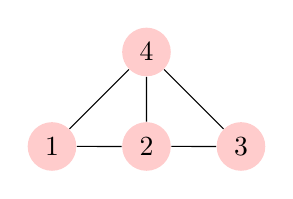
\begin{tikzpicture}
  [scale=.6,auto=left,every node/.style={circle,fill=red!20}]
  \node (n1) at (1,7) {1};
  \node (n2) at (3,7)  {2};
  \node (n3) at (5,7)  {3};
  \node (n4) at (3,9)  {4};

  \foreach \from/\to in {n1/n2,n2/n3,n2/n4,n1/n4,n3/n4}
    \draw (\from) -- (\to);

\end{tikzpicture}
\caption{ Example Graph with 4 vertices and 5 edges}\label{4g1}
\end{center}
\end{figure}

\begin{figure}
\begin{center}
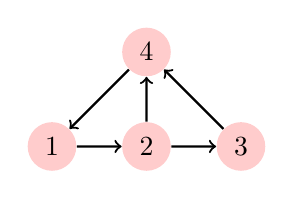
\begin{tikzpicture}
  [scale=.6,auto=left,every node/.style={circle,fill=red!20}]
  \node (n1) at (1,7) {1};
  \node (n2) at (3,7)  {2};
  \node (n3) at (5,7)  {3};
  \node (n4) at (3,9)  {4};

\path [->,draw,thick]
(n2) edge  (n3)
(n3) edge   (n4)
(n4) edge   (n1)
(n1) edge   (n2)
(n2) edge  (n4)
;
\end{tikzpicture}
\caption{ Eulerian Path from vertex 2 to vertex 4 2-3-4-1-2-4 of Figure \ref{4g1}}\label{4g15}
\end{center}
\end{figure}
\vspace{2cm}
Rishnak then asked Ajur whether you can start a walk from vertex 1 to vertex 9 and visit all edges once and only once (Eulerian walk from vertex 1 to vertex 9) in connected graph in Figure \ref{4g2}.
Ajur was perplexed. Then he tried to reason - he can break them into cycles. (2,3,7),(7,6,5,4), (3,4,8)  - None of these cycles had any edge in common. So he constructed a walk as (1,(1,2),2,(2,3),
3,(3,4),4,(4,8),8,(8,3),3,(3,7),7, (7,6),6,(6,5),5,(5,4).4,(4,7),7,
(7,2),2,(2,8),8,(8,9),9). Ajur further explained that he obtained this Eulerian walk by essentially by combining these cycles. He illustrated his walk in Figure \ref{4g25}. Ajur responded that there is no closed Eulerian walk in this graph \ref{4g2} as all the vertices are not of even degree. An Eulerian walk starts from a vertex with odd degree and ends at a vertex with odd degree (There have to be exactly two such vertices).

\begin{figure}
\begin{center}
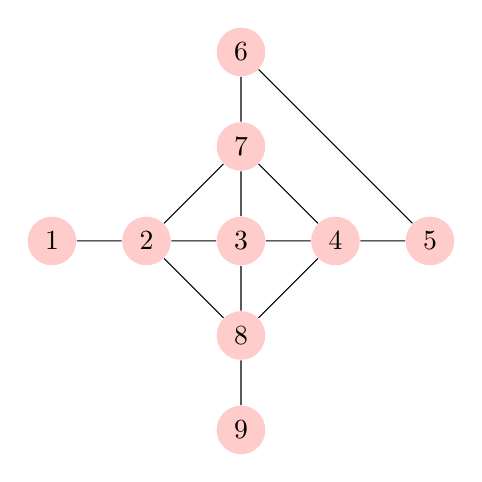
\begin{tikzpicture}
  [scale=.6,auto=left,every node/.style={circle,fill=red!20}]
  \node (n1) at (1,7) {1};
  \node (n2) at (3,7)  {2};
  \node (n3) at (5,7)  {3};
  \node (n4) at (7,7) {4};
  \node (n5) at (9,7)  {5};
  \node (n6) at (5,11)  {6};
   \node (n7) at (5,9) {7};
   \node (n8) at (5,5) {8};
   \node (n9)  at (5,3) {9};
  \foreach \from/\to in {n1/n2,n2/n3,n3/n4,n4/n5,n6/n7,n7/n3,n3/n8,n8/n9,n2/n7,
  n4/n7,n4/n8,n8/n2,n6/n5}
    \draw (\from) -- (\to);

\end{tikzpicture}
\caption{ Example Graph with 9 vertices and 13 edges}\label{4g2}
\end{center}
\end{figure}

\begin{figure}
\begin{center}
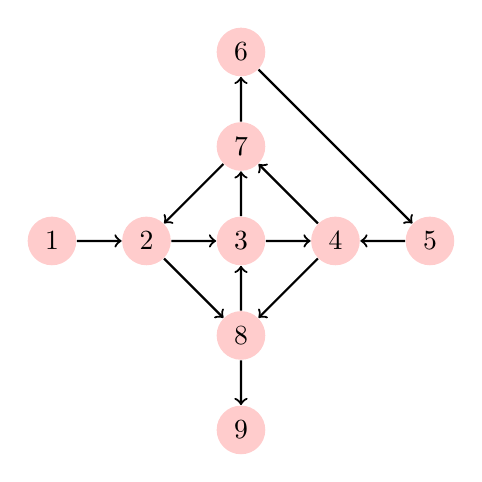
\begin{tikzpicture}
  [scale=.6,auto=left,every node/.style={circle,fill=red!20}]
  \node (n1) at (1,7) {1};
  \node (n2) at (3,7)  {2};
  \node (n3) at (5,7)  {3};
  \node (n4) at (7,7) {4};
  \node (n5) at (9,7)  {5};
  \node (n6) at (5,11)  {6};
   \node (n7) at (5,9) {7};
   \node (n8) at (5,5) {8};
   \node (n9)  at (5,3) {9};
 \path [->,draw,thick] 
  (n1) edge  (n2)
  (n2) edge (n3)
  (n3) edge (n4)
  (n4) edge (n8)
  (n8) edge (n3)
  (n3) edge (n7)
  (n7) edge (n6)
  (n6) edge (n5)
  (n5) edge (n4)
  (n4) edge (n7)
  (n7) edge (n2)
  (n2) edge (n8)
  (n8) edge (n9)
;
\end{tikzpicture}
\caption{ Eulerian Walk from vertex 1 to vertex 9  1-2-3-4-8-3-7-6-5-4-7-2-8-9 of Figure \ref{4g2}}\label{4g25}
\end{center}
\end{figure}

\vspace{3in}
Rishnak asked Ajur how would you make the graph shown in Figure \ref{4g2} to have a closed Eulerian Walk. Ajur reasoned that there are exactly two vertices of odd degrees, namely, vertices 1 and 9. If we join an edge between 1 and 9,  every vertex will have an even degree and hence a closed Eulerian Walk and that walk will be 1-2-3-4--8--7-6-5-4-7-2-8-9-1. Ajur also drew a graph.

\begin{figure}
\begin{center}
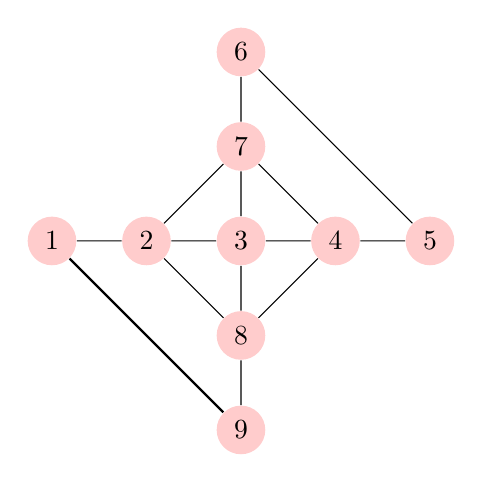
\begin{tikzpicture}
  [scale=.6,auto=left,every node/.style={circle,fill=red!20}]
  \node (n1) at (1,7) {1};
  \node (n2) at (3,7)  {2};
  \node (n3) at (5,7)  {3};
  \node (n4) at (7,7) {4};
  \node (n5) at (9,7)  {5};
  \node (n6) at (5,11)  {6};
   \node (n7) at (5,9) {7};
   \node (n8) at (5,5) {8};
   \node (n9)  at (5,3) {9};
  \foreach \from/\to in {n1/n2,n2/n3,n3/n4,n4/n5,n6/n7,n7/n3,n3/n8,n8/n9,n2/n7,
  n4/n7,n4/n8,n8/n2,n6/n5}
    \draw (\from) -- (\to);
\path[thick] (n1) edge (n9);
\end{tikzpicture}
\caption{ Closed Eulerian Walk with edge (1,9) added to Figure \ref{4g2}}\label{4g255}
\end{center}
\end{figure}

Rishnak asked how will you make graph shown in Figure \ref{4g1} to have a closed Eulerian walk. Ajur now had a problem. The two vertices which have odd degrees 2 and 4, already have an edge between them. However, he remembered the definition of a multigraph, where in between any two vertices, there can be more than one edge. So he added another edge between 2 and 4 and there is a closed Eulerian walk 2-3-4-1-2-4-2. Ajur again drew a graph as shown in Figure \ref{4g155}
Ajur added that if a graph is not connected, there is neither Eulerian walk nor a closed Eulerian walk.
\begin{figure}
\begin{center}
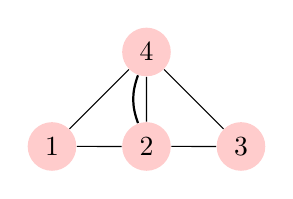
\begin{tikzpicture}
  [scale=.6,auto=left,every node/.style={circle,fill=red!20}]
  \node (n1) at (1,7) {1};
  \node (n2) at (3,7)  {2};
  \node (n3) at (5,7)  {3};
  \node (n4) at (3,9)  {4};

  \foreach \from/\to in {n1/n2,n2/n3,n2/n4,n1/n4,n3/n4}
    \draw (\from) -- (\to);
\path[thick] (n2) edge[bend left=20] (n4);
\end{tikzpicture}
\caption{ Graph in Figure \ref{4g1} with edge (2,4) added to have a closed Eulerian Walk}\label{4g155}
\end{center}
\end{figure}

\vspace{3in}
Rishnak asked Ajur whether he knew about multi graphs and directed graphs. Ajur realized he essentially learnt about multigraphs  by doing Eulerian walks and completion  example. Ajur added that in a directed graph an edge $(x,y)$ goes from vertex $x$ to $y$ and he drew an example graph to show Rishnak that he knows. See Figure \ref{4g5}. Ajur mentioned that instead of degree of a vertex, we have in-degree and out-degree of a vertex. The number of edges coming to a vertex is the in-degree of that vertex and the number of edges going out of a vertex is the out-degree of a vertex. For example, in the directed graph shown in Figure \ref{4g5}, vertex 1 has in-degree 2 and out-degree 1. Each of Vertex 3 and 4 has in-degree  and out-degree 1. A directed graph is strongly connected if there is a directed path from every vertex to every other vertex. For example, directed graph shown in Figure \ref{4g5} is strongly connected. 
\begin{figure}
\begin{center}
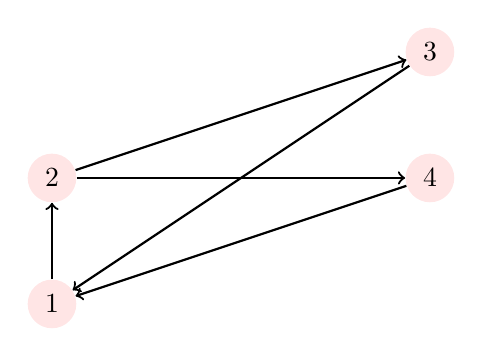
\begin{tikzpicture}
  [scale=.8,auto=left,every node/.style={circle,fill=red!10}]
  \node (n1) at (1,7) {1};
  \node (n2) at (1,9)  {2};
  \node (n3) at (7,11)  {3};
  \node (n4) at (7,9) {4};
 \path[->, draw,thick] 
        (n1) edge (n2)
         (n3) edge (n1)
        (n2) edge (n3)
        (n2) edge (n4)
        (n4) edge  (n1);

\end{tikzpicture}
\caption{ Example Directed Graph with 4 vertices and 5 edges}\label{4g5}
\end{center}
\end{figure}

Anticipating what Rishnak is going to ask, Ajur responded by saying that there is no closed Eulerian walk in this directed graph. Rishnak reminded that he wanted whether Ajur knew an Euler walk from vertex 2 to vertex 1. Ajur reasoned in a  manner similar to what he did before. Ajur saw a directed cycle (1,(1,2),2,(2,3),3,(3,1),1) or simply (1,2,3,1). So Ajur was able to write the Eulerian walk as 2-3-1-2-4-1. Ajur said to have a closed Eulerian walk, you should have a collection of edge disjoint cycles (no edge is common between these cycles). In such a case, the in-degree of each vertex should be the same as its out-degree (this is similar to the degree of every vertex has to be even number as in the case of undirected graphs). For an Eulerian walk, it has to start from a vertex which has one more out-degree than in-degree and end in a vertex which has one more in-degree than out-degree (For all other vertices, in-degree should be equal to out-degree).

Rishnak saw it is getting late - but wanted to share some exciting applications of Eulerian walks. 
Suppose the question is to obtain a string 0's and 1's such that all four two bit strings occur as a substring (there are 4 two bit strings consisting of 0's and 1's namely 00,01,10 and 11). For example if you have 0011 - all two bit strings occur as a substring namely 00, 01, 11 and 10. If it were a circular string then 0011 will suffice to get all 4 two bit strings. Rishnak added that this problem is closely related to closed Eulerian walk. If we construct an Eulerian walk on this directed graph \ref{4g55}, we will get that string.

For this directed graph, there are two verticee with labels 0 and 1 . There is a directed edge with label 0 from vertex labeled 0 to itself. There is a directed edge with a label 1 from vertex labeled 0 to a vertex labeled 1. (The idea behind the first edge is to consider appending 0 (edge label) to 0 (the starting vertex label) get 00. Then omit the first character 0. The result is 0 which is the vertex labeled 0 - hence a self loop). Similarly there is an edge with a label 1 from a vertex labeled 1 to itself and there is a vertex an edge with 
a label 0 from vertex labeled 1 to a vertex labeled 0.
Each vertex has an in-degree of 2 and an out-degree if 2. Hence it has a closed Eulerian walk from a vertex labeled 0 to itself and that walk is 0110 (all of them are edge labels). From this, we get all the four substrings of length 2, namely 01,11,10,00 (the last one is taking the last character and the first character as it is a closed walk).

\begin{figure}
\begin{center}
\begin{tikzpicture}[shorten >=1pt,node distance=4cm,on grid,auto] 
 
   \node[state] (q_1)  {$0$}; 
   \node[state] (q_2) [below =of q_1] {$1$}; 
    \path[->,draw,thick] 
    
    (q_1) edge [bend left=15] node  {1} (q_2)
          edge [loop above] node {0} ()
    (q_2) edge [bend left=15] node [swap] {0} (q_1) 
          edge [loop below] node {1} ();
   
\end{tikzpicture}
\caption{ An Eulerian walk on this directed graph will yield a DeBruijn sequence to obtain all substrings of length 2 over a binary alphabet 0 and 1}\label{4g55}
\end{center}
\end{figure}

Suppose the question is to obtain a string 0's and 1's such that all eight three bit strings occur as a substring (there are 8 three bit strings consisting of 0'1 and 1's namely 000,001,010,011,100,101,110,111). Such a string is known as deBruijn string!  Consider a directed graph with 4 vertices (labeled 00, 01, 10 and 11).
There is an edge from vertex labeled 00 to itself with a label 0 (if you get a 0, you append 0 to the vertex label (00) and drop the first character). There is an edge with label 1 from
vertex labeled 00 to a vertex labeled 01. Vertex labeled 00 has an out-degree of 2. Similarly draw an edge with label 0 from vertex labeled 01 to vertex with label 10. Draw an edge with label 1 from vertex labeled 01 to vertex with label 11. 
Draw an edge with label 0 from a  vertex labeled 10 to a vertex labeled 00. Draw an edge with label 1 from a vertex labeled 10 to a vertex labeled 01.
Draw an edge with label 0 from a vertex labeled 11 to a vertex labeled 10. Draw an edge with label 1 from a vertex labeled 11 to itself.
The resulting directed graph is as shown in Figure \ref{4g6}. An Eulerian walk starting from a vertex labeled 00 is $0 1 0 1 1 1 0 0$  (We start with a vertex labeled 00 and the label of the edges traversed in an Eulerian Walk). This walk is also a closed Eulerian Walk as we start and end with the same vertex (labeled $00$).
From the walk, we get all the strings of length 3 (over 0 and 1) as substrings in the Eulerian Walk.
001, 010,101,011,111,110,100 and 000 (000 by knowing this is a closed Eulerian walk and we get 000, by taking two characters and the first character of the Eulerian Walk.).
\begin{figure}
\begin{center}
\begin{tikzpicture}[shorten >=1pt,node distance=4cm,on grid,auto] 
   \node[state] (q_0)   {$10$}; 
   \node[state] (q_1) [above right=of q_0] {$00$}; 
   \node[state] (q_2) [below right=of q_0] {$11$}; 
   \node[state](q_3) [below right=of q_1] {$01$};
    \path[->,draw,thick] 
    (q_0) edge  node {0} (q_1)
          edge [bend left=15] node  {1} (q_3)
    (q_1) edge  node  {1} (q_3)
          edge [loop above] node {0} ()
    (q_2) edge  node [swap] {0} (q_0) 
          edge [loop below] node {1} ()
    (q_3) edge [bend left=15] node [swap] {0} (q_0) 
          edge  node [swap] {1} (q_2);
\end{tikzpicture}
\caption{ An Eulerian walk on this directed graph will yield a DeBruijn sequence to obtain all substrings of length 3 over a binary alphabet 0 and 1}\label{4g6}
\end{center}
\end{figure}

